\chapter{Data Description}


Con el fin del modelado del sistema completo del invernadero describiremos las bases de datos disponbiles de este. Como veremos tenemos una gran cantidad de información en las variables de clima, mientras que las medidas  crecimiento de la plantación se reduce a la producción del fruto. Además procederemos a explicar un pre-procesado preliminar que podemos realizar sin necesidad de tener en cuenta los modelos de clima, ni de crecimientos. Este constará de un eliminación de ruido y una pre selección de variables con información relevante

\section{Available data}


El invernadero cosnta de un sistema de captura de datos llamado \emph{sysclima}, enfocado en las variables climáticas, a continuación la describiremos la base de datos capturado por \emph{sysclima}. 

\begin{dataset}[SysClima]\label{dataset:sysclima}
Serie temporal de variables climáticas con una frecuencia de muestreo de aproximadamente $2$ minutos. Además de las variables de clima esta base de datos contiene información sobre el estado de la pantalla de sombreo y del porcentaje de apertura de las ventanas, variables que podemos considerar como variables manipulables. Mostramos una descripción detallada de las variables en la tabla \ref{table:SysClimaDS} y una representación gráfica en la Figura \ref{fig:ViewDataSetSysClima}.
\end{dataset}

Estos datos en bruto contienen muchas variables que son dependientes debido a que el sistema sysclima los computa. Es decir, existen variables como por ejemplo la temperatura de rocío (\texttt{Troco}) que son calculados a partir de una formula utilizada por el sistema. Removeremos este tipo de variables dado que estamos interesados en encontrar las correlaciones entre las medidas independientes. Por otra parte, tambien removeremos variables cuyo valor sea constante, dado que no aporta información relevante. Siguiendo estos pasos obtenemos la siguiente base de datos:

\begin{dataset}[SysClima Compact]\label{dataset:sysclima2}
    Serie Temporal con menos de variables que la base de datos \ref{dataset:sysclima}. Se puede ver 
\end{dataset}

Aunque esta es una base de datos con una buena resolución, esta contiene ventanas temporales sin datos de longitud aproximada de varias semanas. Aunque para el modelado de la temperatura interior, este nos es un problema; el modelado del crecimiento de la plantación depende fuertemente las condiciones climaticas en ventanas de tiempo del orden de meses. La falta de datos en la base de datos \ref{dataset:sysclima} nos imposibilita el uso de modelos mecanísticos para la predicción de la producción. Es por ello que hemos recogido los datos meteorológicos de la estación más cercana con registros históricos, que a continuación describiremos.

\begin{dataset}[Meteorologic Station of Derio - Euskalmet]\label{dataset:Euskalmet}
    Serie temporal de variables climática de la estación meteorológica de Derio, desde 2016 hasta 2020. Utilizaremos esta base de datos de clima con el fin de complementar las regiones sin medidas de la base de datos \ref{dataset:sysclima}.
\end{dataset}

Esta base de datos contiene información de la temperatura sin grandes ventanas vacias, sin embargo existe una ausencia de datos de radiación en el intervalo XXXX-YYYY. 

Por otro lado, como hemos mencionado anteriormente el único registro claro con respecto al crecimiento de la plantación la masa de fruto recogido. Este registro se encuentra en la siguiente base de datos.

\begin{dataset}[Tomatoes Production] 
    Serie temporal de masa de tomates producidos con una frecuencia de muestreo aproximada diaria. Estos datos son recogidos manualmente por el personal del invernadero.
\end{dataset}


\def\myarray{ Time Stamp    /   -               /                           , 
              Var2          /   $-$             /  Greenhouse Sector        ,
              Textt         /   $^\circ C$      /  Exterior Temperature     ,
              HRExt         /   $W/m^2$         /  Humedad relativa Exterior,
              RadExd        /   $W/m^2$         /  Exterior Radiation       }



\begin{table}
    \centering
    \begin{tabular}{|c|c|c|c|}
        \hline
        \textbf{Name}           & \textbf{Units} & \textbf{Description}         \\ 
        \hline
        \texttt{Time Stamp}         & -              &                              \\ \hline
        \texttt{Var2}               & -              & Sección de invernadero       \\ \hline
        \texttt{Text}               & $^\circ C$     & Temperatura exterior         \\ \hline
        \texttt{HRExt}              & \%             & Humedad relativa Exterior    \\ \hline
        \texttt{RadExt}             & $W/m^2$        & Radiación Exterior           \\ \hline
        \texttt{Vviento}            & $km/s$         & Wind Velocity         \\  \hline
        \texttt{DireccinViento}     & $^\circ$       & Dirección del Viento         \\ \hline
        \texttt{RadAcumExt}         & $W/m^2$        & Radiación Acumulada diaria Exterior \\ \hline
        \texttt{AlarmaLluvia}       & -              & Alarma de Viento             \\ \hline
        \texttt{AlarmaVto}          & -              & Alarma de Lluvia             \\ \hline
        \texttt{Tinv}               & $^\circ C$     & Temperatura interior         \\ \hline
        \texttt{Troco}              & $^\circ C$     & Temperatura de Rocio\\  \hline
        \texttt{RadInt}             & $W/m^2$        & Radiación Interior \\ \hline
        \texttt{xDemPant1}          & $\%$           & Demanda de Pantalla de Sombreo\\ \hline
        \texttt{xEstadoPant1}       & $\%$           & Estado de Pantalla de Sombreo\\ \hline
        \texttt{TVentilacin}        & $^\circ C$     & Temperatura de Ventilación \\ \hline
        \texttt{EstadoCenitalE}     & $\%$           &       \\ \hline
        \texttt{EstadoCenitalO}     & $\%$           & \\ \hline
        \texttt{EstadoLateralE}     & $\%$           & \\ \hline
        \texttt{MaxHR}              & $\%$           & \\ \hline
        \texttt{MinHR}              & $\%$           & \\ \hline
        \texttt{DeltaX}             & $g/m^3$        & \\ \hline
        \texttt{DeltaT}             & $^\circ C$     &  \\ \hline
        \texttt{DPV}                & $mbar$         & Déficit de Presión de Vapor \\  \hline
        \texttt{HRInt}              & $\%$           &  \\ \hline
        \texttt{Ventiladores2Activo}& &  \\ \hline
        \texttt{Aerotermo1Activo} & &\\ \hline
        \texttt{Sonda1} & & \\ \hline
        \texttt{Sonda2} & & \\ \hline
        \texttt{Sonda3} & & \\ \hline
        \texttt{Sonda5} & & \\ \hline
        \texttt{Sonda6} & & \\
        \hline
    \end{tabular}
    \caption{Variables of dataset \ref{dataset:sysclima}}
    \label{table:SysClimaDS}
\end{table}



\begin{table}
    \centering
    \begin{tabular}{|c|c|c|c|}
        \hline
        \textbf{Name}           & \textbf{Units} & \textbf{Description}         \\ \hline
        \texttt{Var2}           & -              & Sección de invernadero       \\ \hline
        \texttt{Text}           & $^\circ C$     & Temperatura exterior         \\ \hline
        \texttt{HRExt}          & \%             & Humedad relativa Exterior    \\ \hline
        \texttt{RadExt}         & $W/m^2$        & Radiación Exterior           \\ \hline
        \texttt{Sonda6} \\
        \hline
    \end{tabular}
    \caption{Variables of Dataset \ref{}}
    \label{table:Euskalmet}
\end{table}


\begin{figure}[ht!]
    \centering
    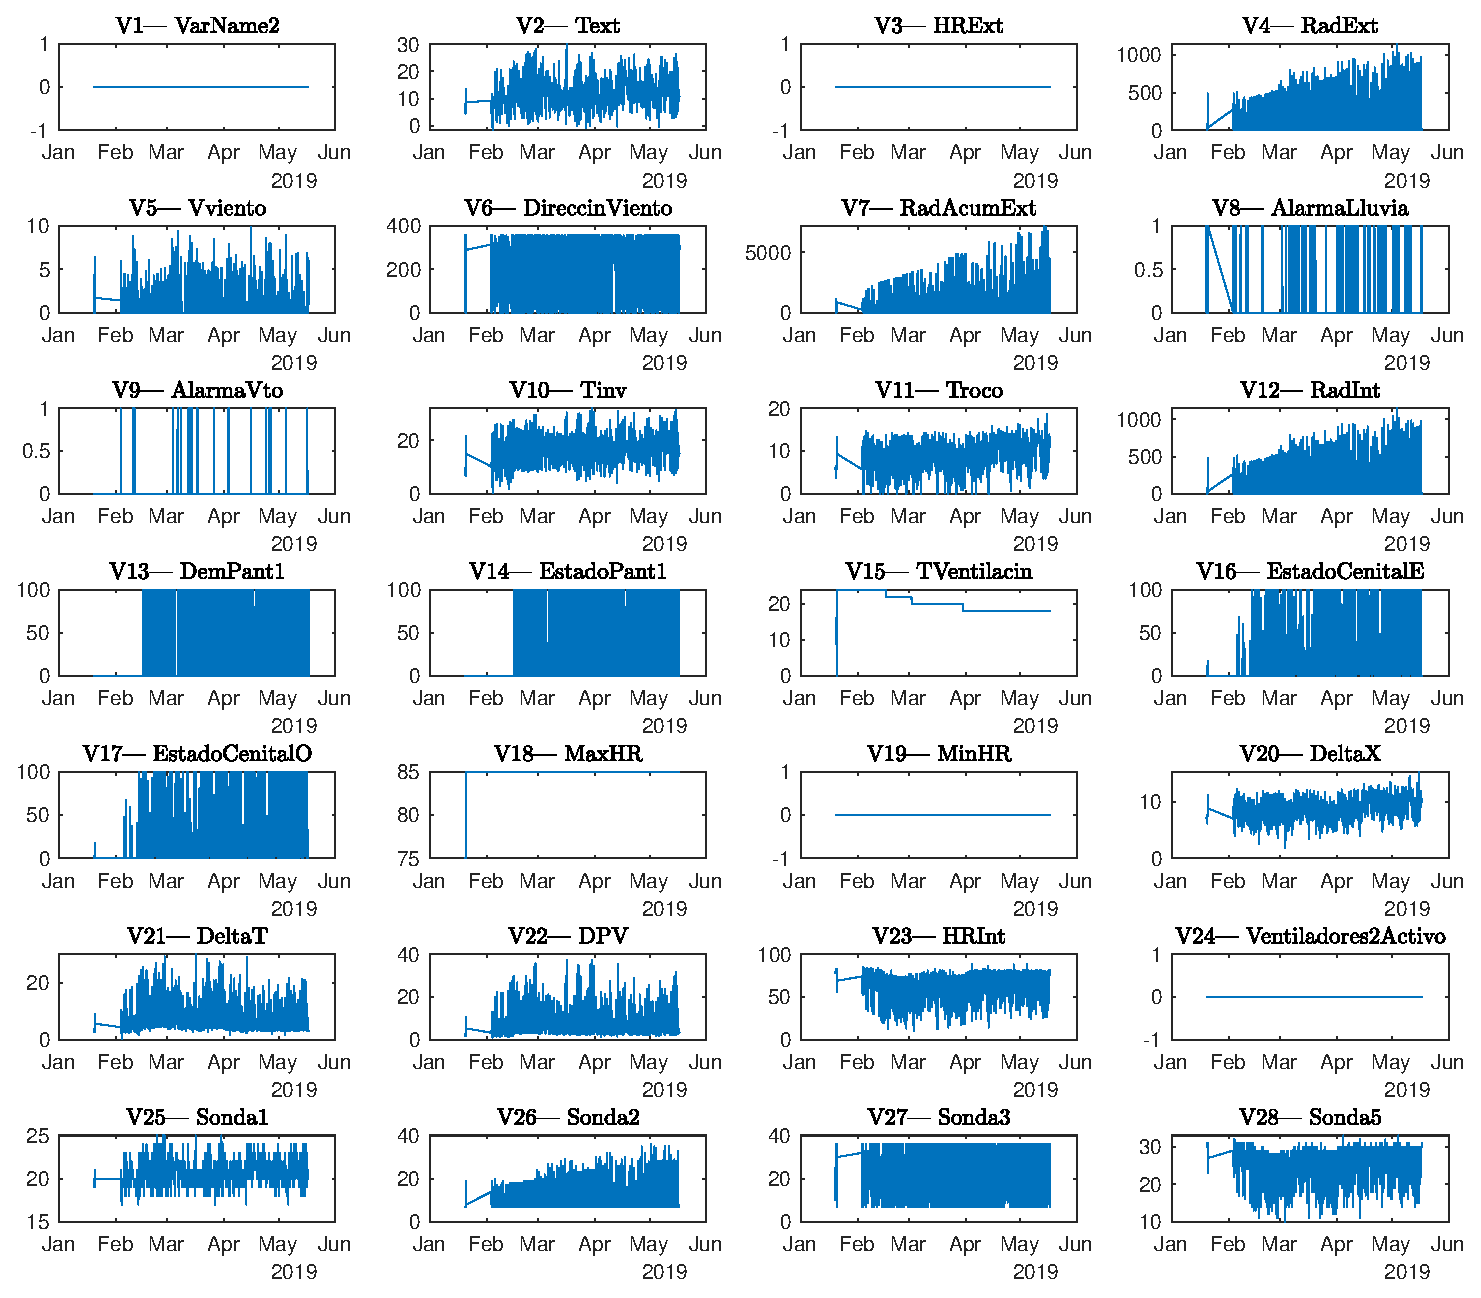
\includegraphics[scale=0.65]{img/fulldata.eps}
    \caption{Preliminary view of Dataset \ref{dataset:sysclima} from Jan-2019 to Jun-2019 }
    \label{fig:ViewDataSetSysClima}
\end{figure}

\begin{figure}
    \centering
    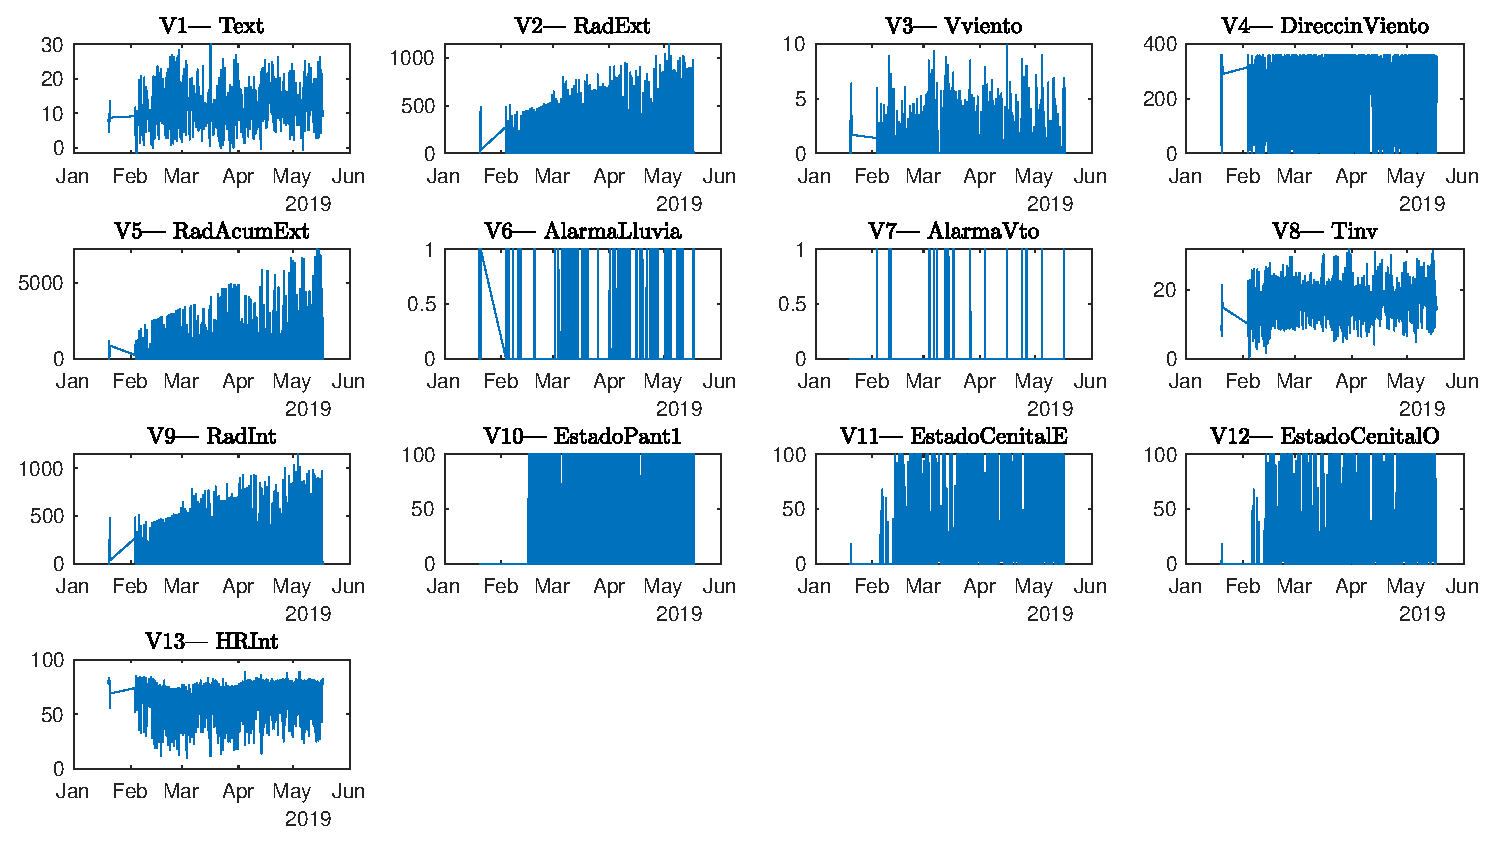
\includegraphics[scale=0.55]{img/fulldata_remove_no_data.eps}
    \caption{Selection of variables}
\end{figure}
\begin{figure}
    \centering
    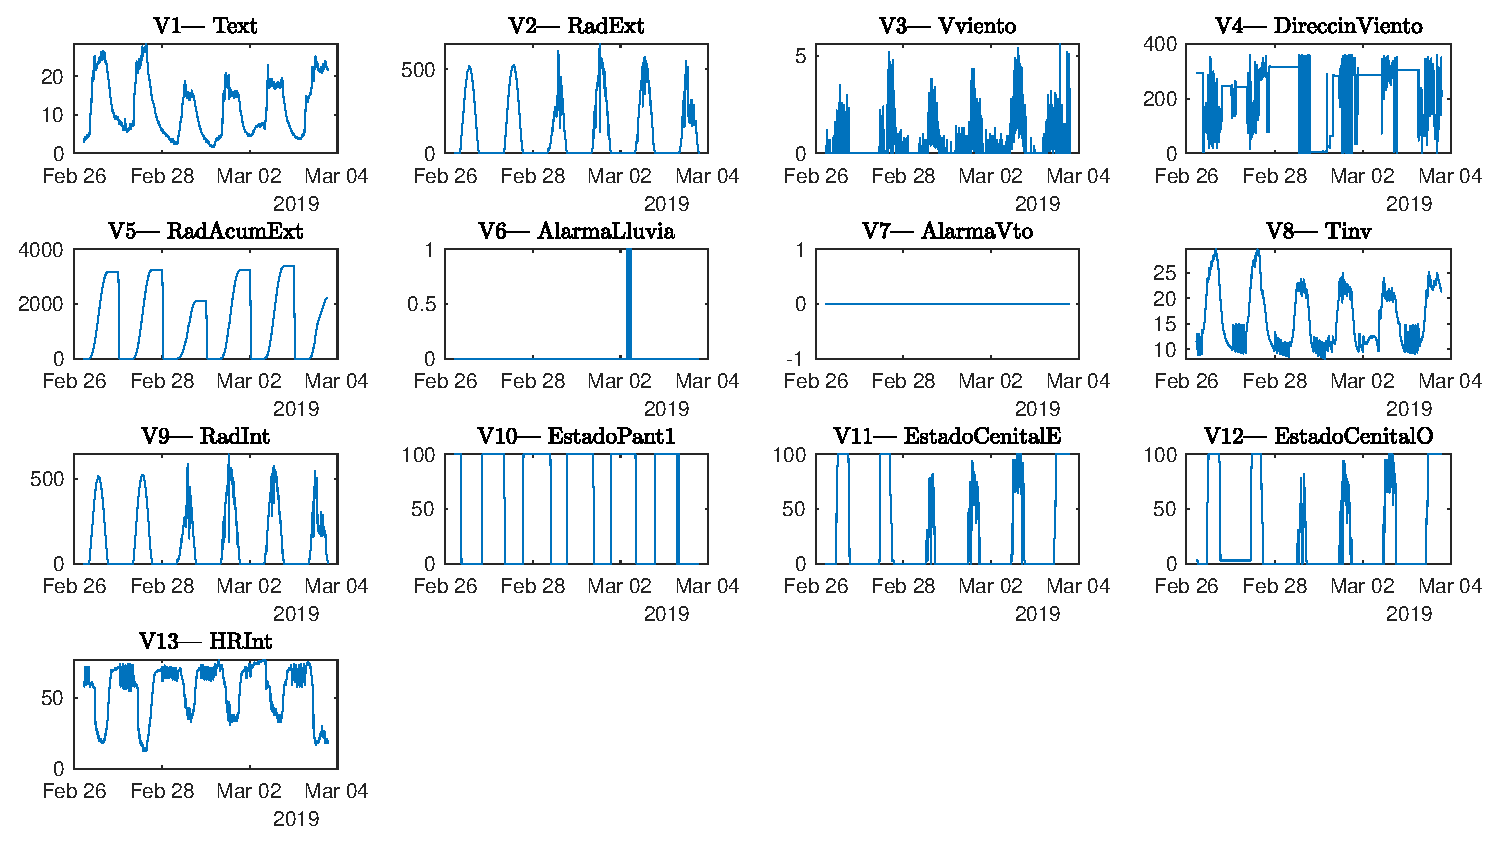
\includegraphics[scale=0.55]{img/fulldata_remove_no_data_zoom.eps}
    \caption{Selection of variables - zoom }
\end{figure}


\section{Análisis estadístico de las bases de datos}


\section{Conclusion}